\begin{frame}

\begin{columns}[onlytextwidth]
    \begin{column}{0.45\textwidth}
    	\textbf{Improvements for electromagnetic interactions:}
    	\begin{itemize}
    		\item Inclusion of $\gamma \to \mu^+ \mu^-$
    		\item Inclusion of $\gamma \to \text{Hadrons}$ \\(Photohadronic interaction)
            \begin{itemize}
                \item[$\rightarrow$] Relevant for very-high energies
            \end{itemize}
    		\item Sampling of deflection angles for bremsstrahlung photons
    		%\item Inclusion of photoelectric interactions of $\gamma$ in preparation
    	\end{itemize}

    	%\hspace{10pt} $\Rightarrow$ More about this later!

    \end{column}
    \begin{column}{0.55\textwidth}

    \begin{figure}
    	\centering
        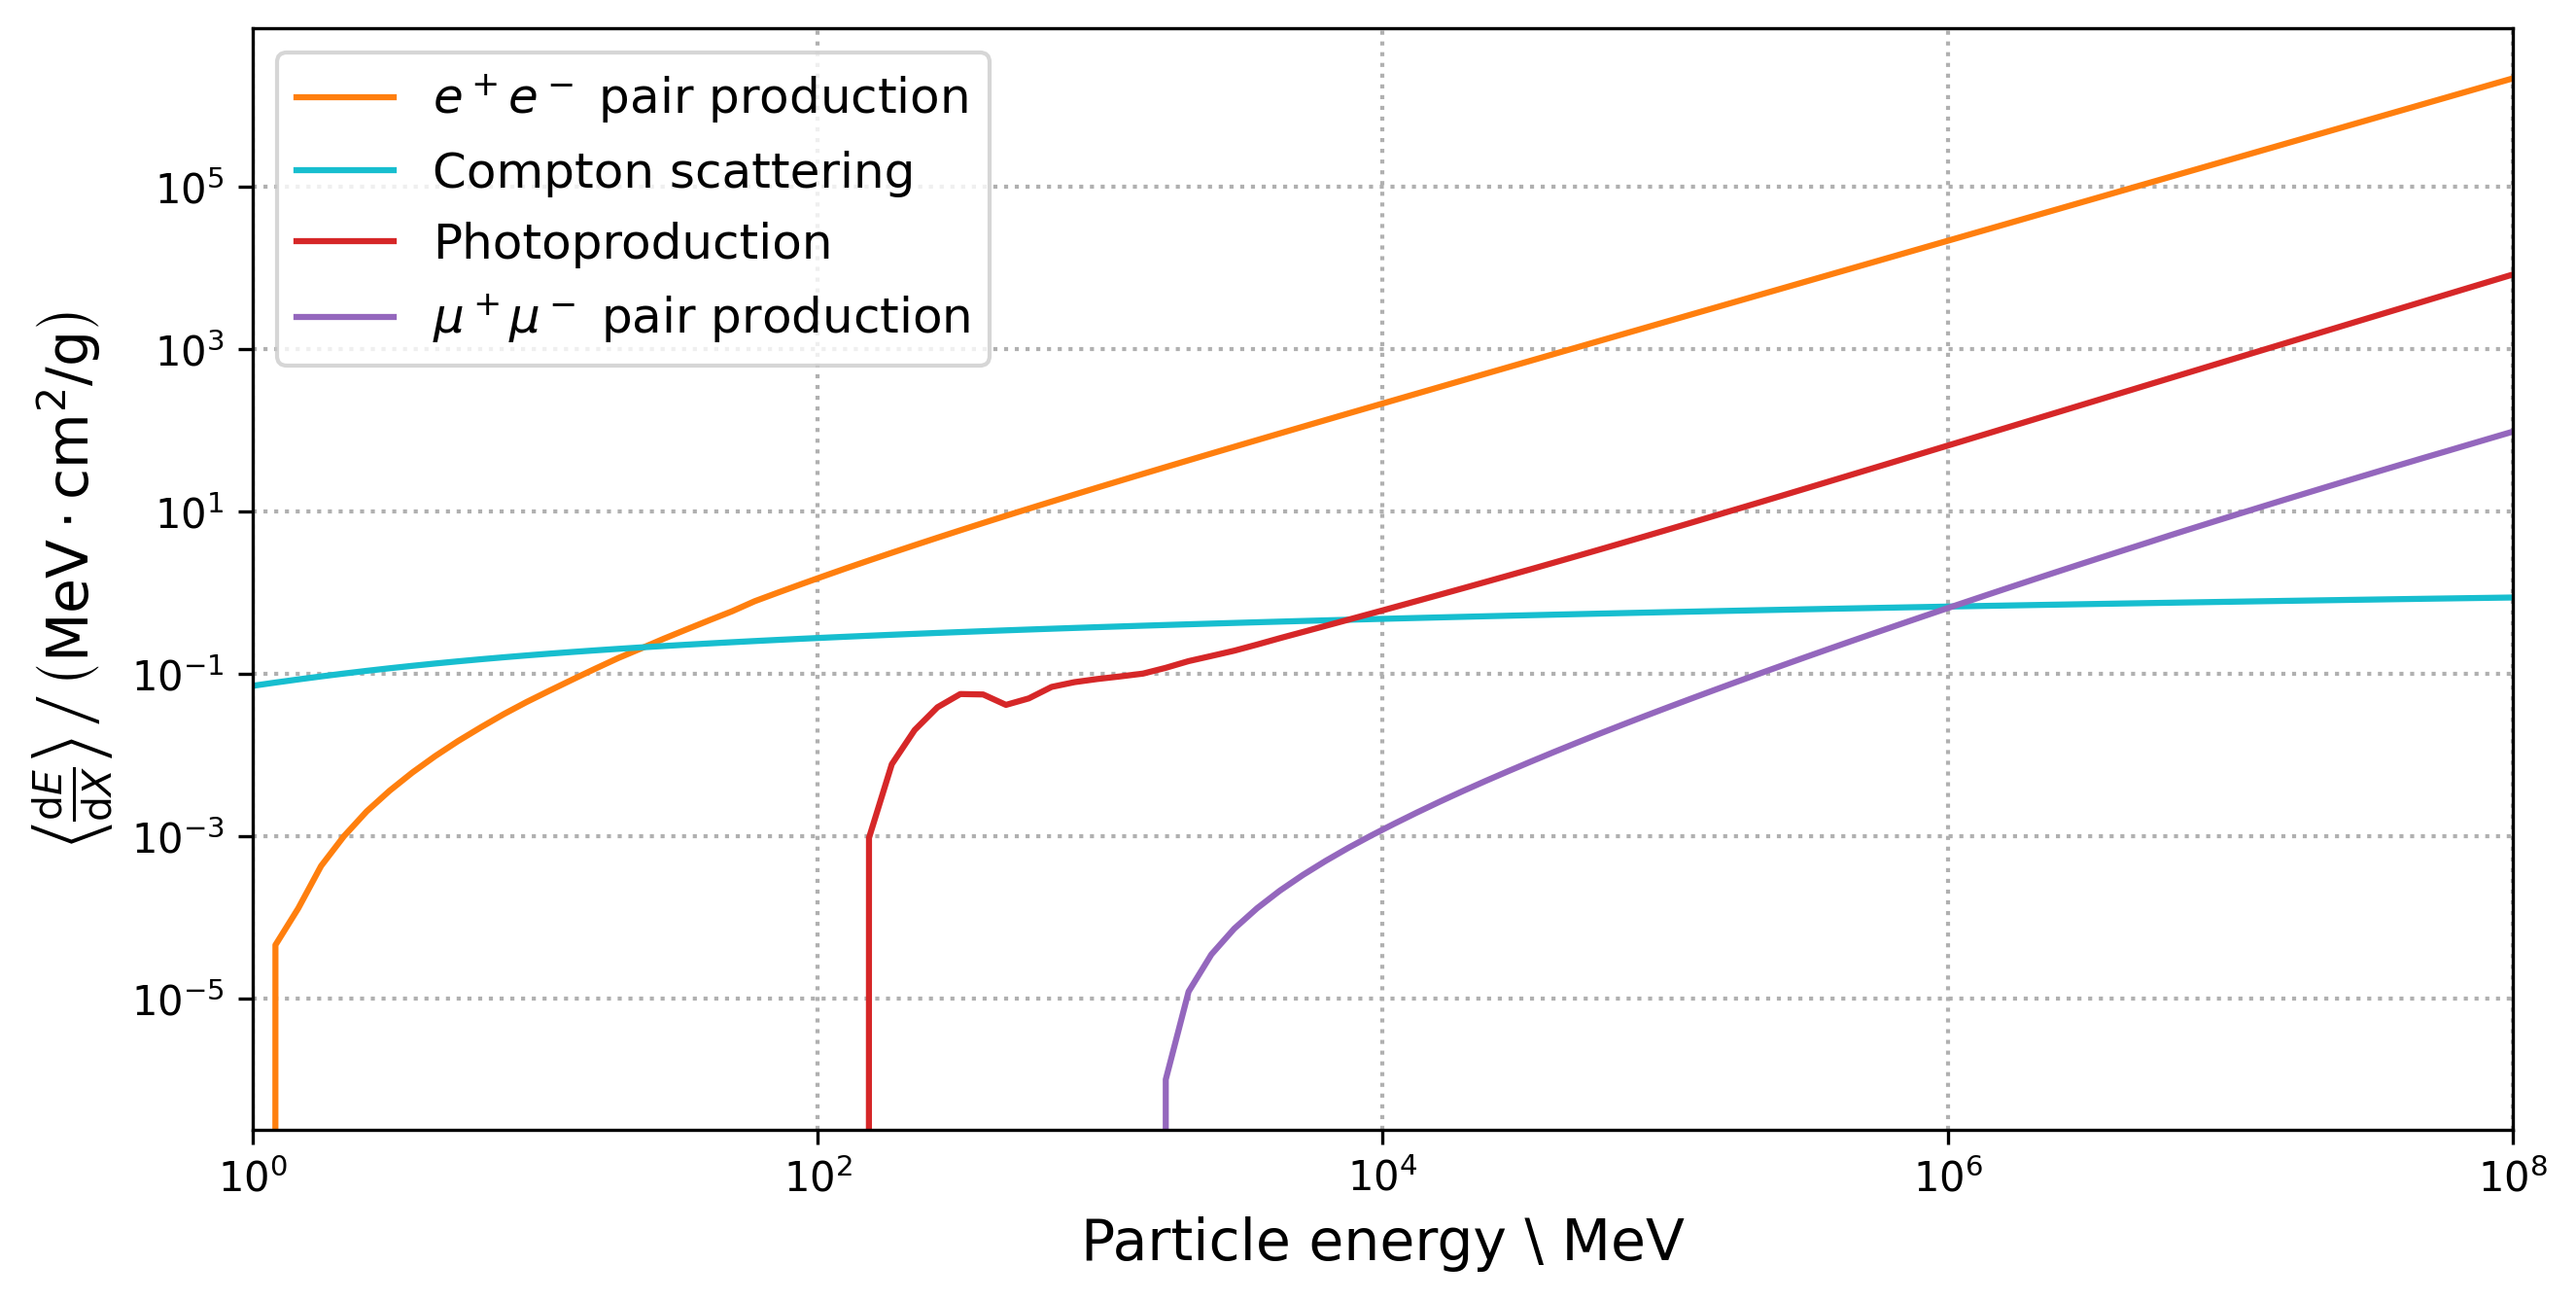
\includegraphics[width=0.9\textwidth]{plots/photon_dEdx.png}
    \end{figure}
    \vspace{-3mm}
    \begin{figure}
        \centering
        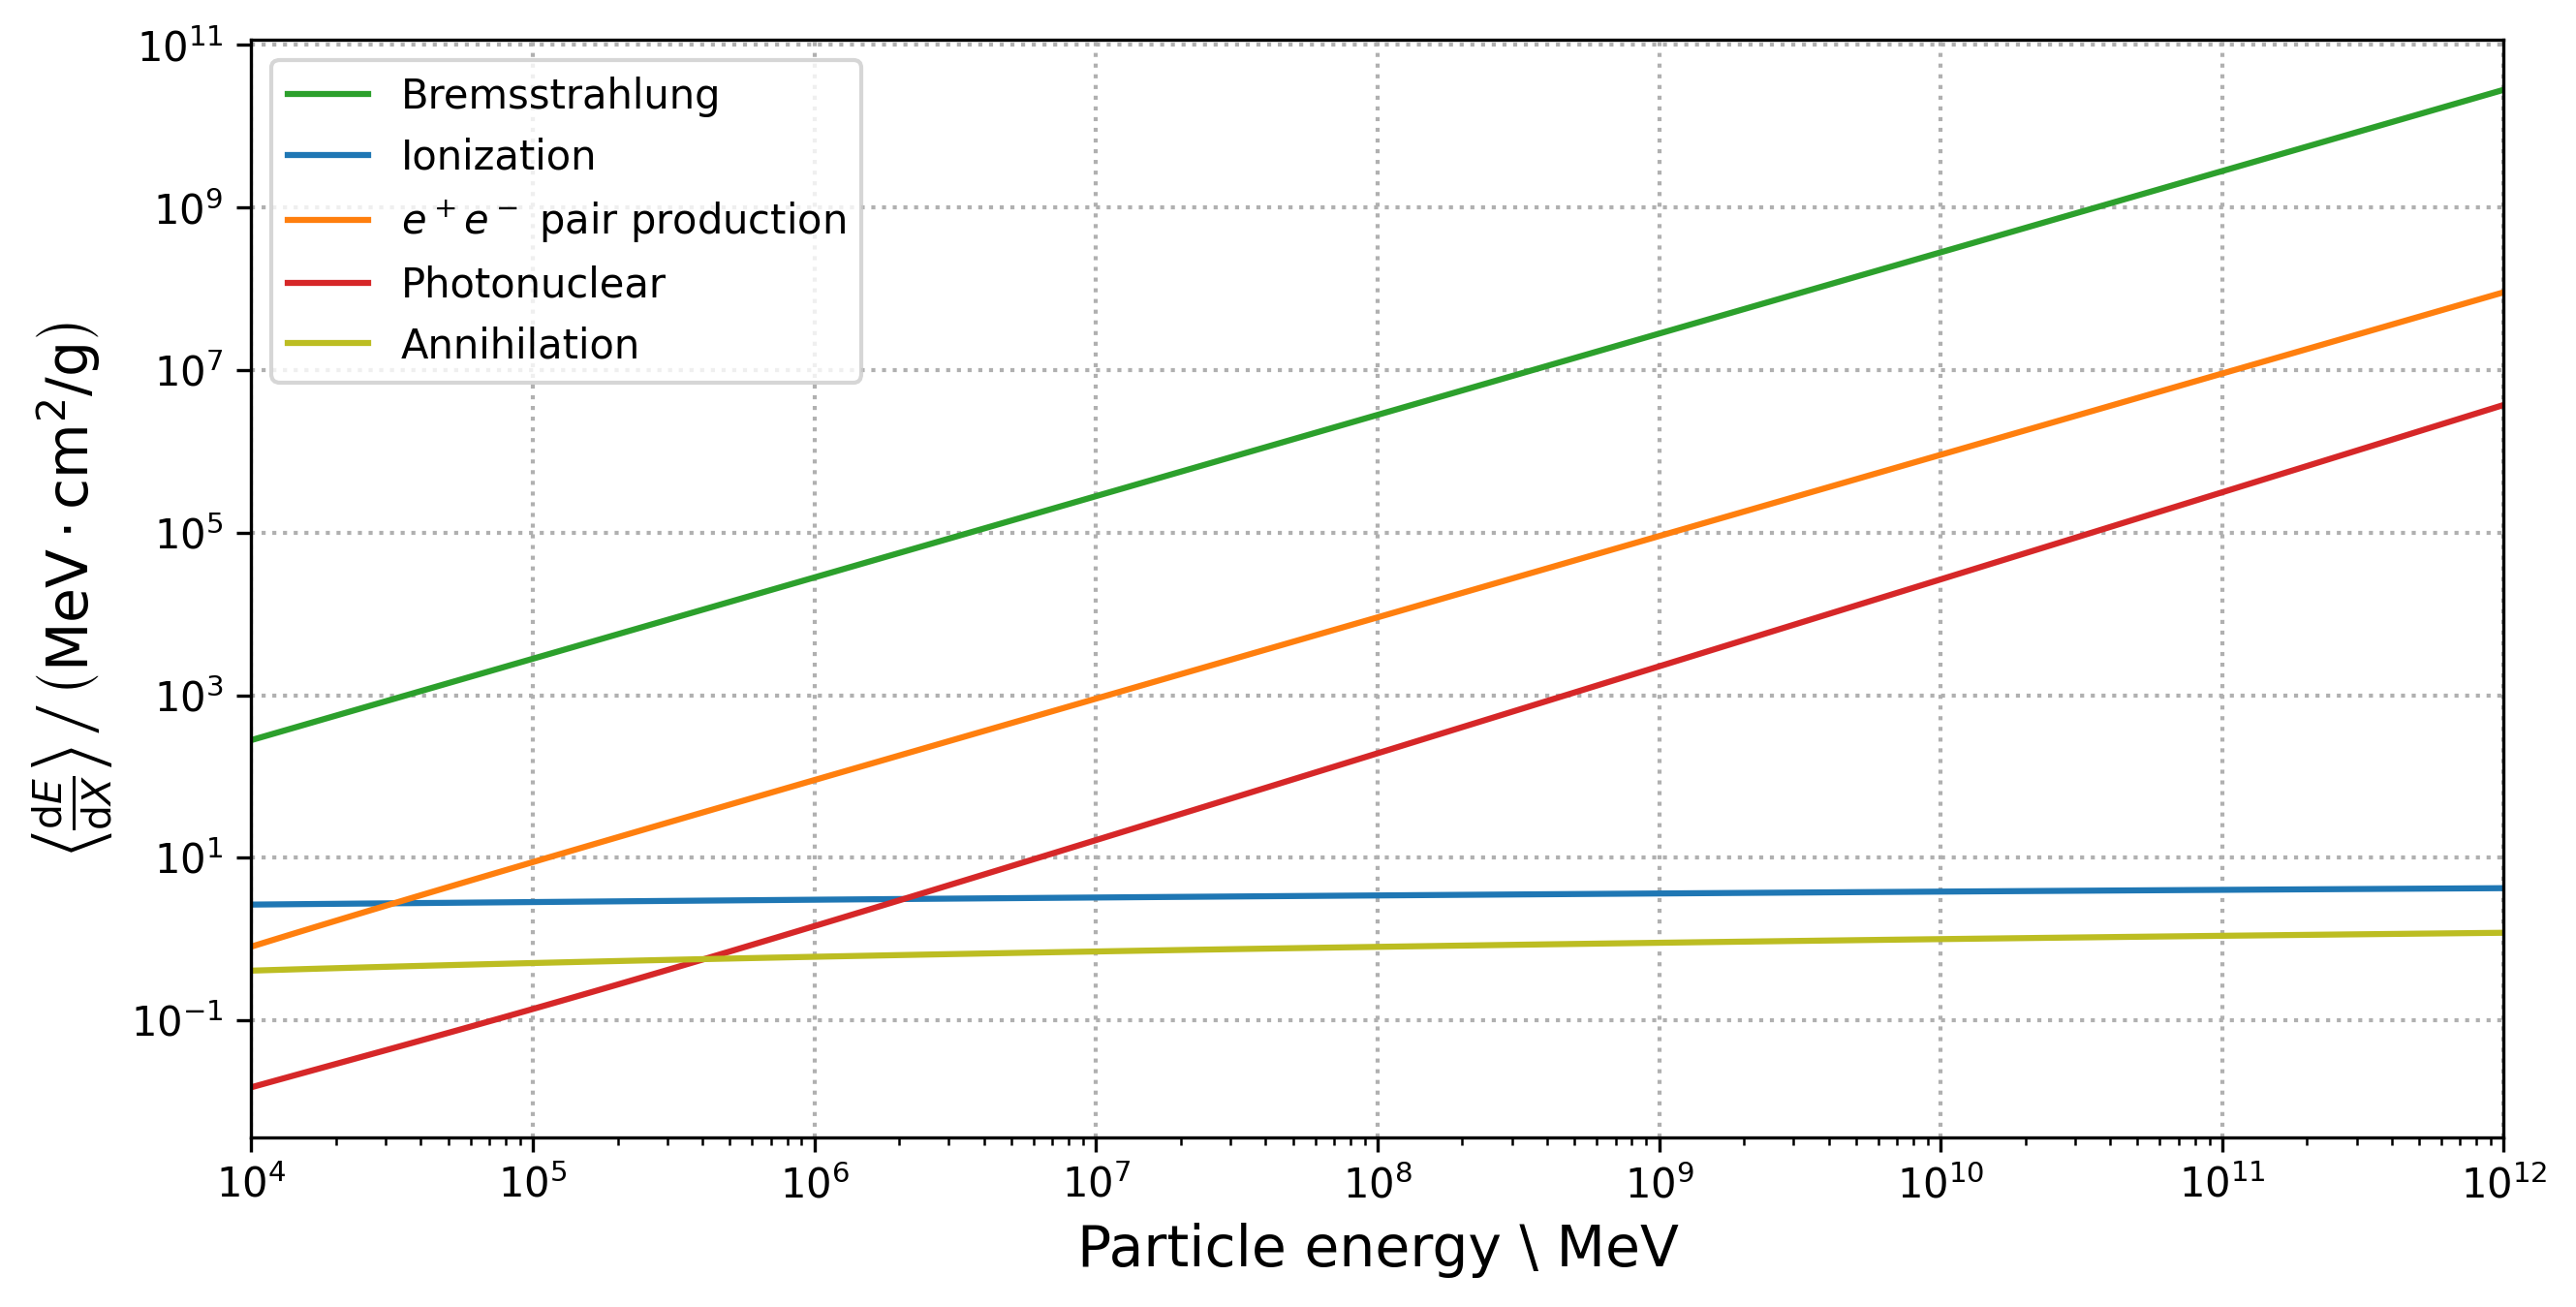
\includegraphics[width=0.9\textwidth]{plots/positron_dEdx.png}
    \end{figure}

    \end{column}
\end{columns}

\end{frame}

\begin{frame}[c]
    \begin{columns}[onlytextwidth]
    \begin{column}{0.45\textwidth}
        \textbf{Stochastic deflections}
        \begin{itemize}
        	\item PROPOSAL considers multiple scattering (continuous losses)
            \item Deflections may also occur in (very) stochastic interactions% (especially for bremsstrahlung and photonuclear interactions)
            \begin{itemize}
            	\item[$\rightarrow$] Possible influence on directional reconstructions?
            \end{itemize}
            \item Stochastic deflections for muon interactions have been added to PROPOSAL
        \end{itemize}
		\vspace{4mm}
        \begin{figure}
            \begin{tikzpicture}[scale=0.7, every node/.style={scale=0.7}]
                \centering

                \coordinate (start) at (-1,0);
                \coordinate (kink) at (1.8, 0);
                \coordinate (end) at (4.5, 0.8);
                \coordinate (continue) at (4.5, 0);



                \draw [black, line width=0.6mm] (start) -- node[above] {$\mu$}  (kink);
                \draw [->, black, line width=0.6mm] (kink) -- node[above] {$\mu^\prime$}  (end);
                \draw [black, dashed, line width=0.2mm] (kink) -- (continue);

                \fill [red] (kink) circle (0.15) node[label=below: $\substack{\text{stochastic} \\ \text{interaction}}$]{};

                \pic [draw, "$\theta$", angle eccentricity=0.7, angle radius=2cm] {angle = continue--kink--end};

            \end{tikzpicture}
        \end{figure}  

    \end{column}
        \begin{column}{0.55\textwidth}
    		\begin{figure}
    		  %\vspace{-9pt}
    		  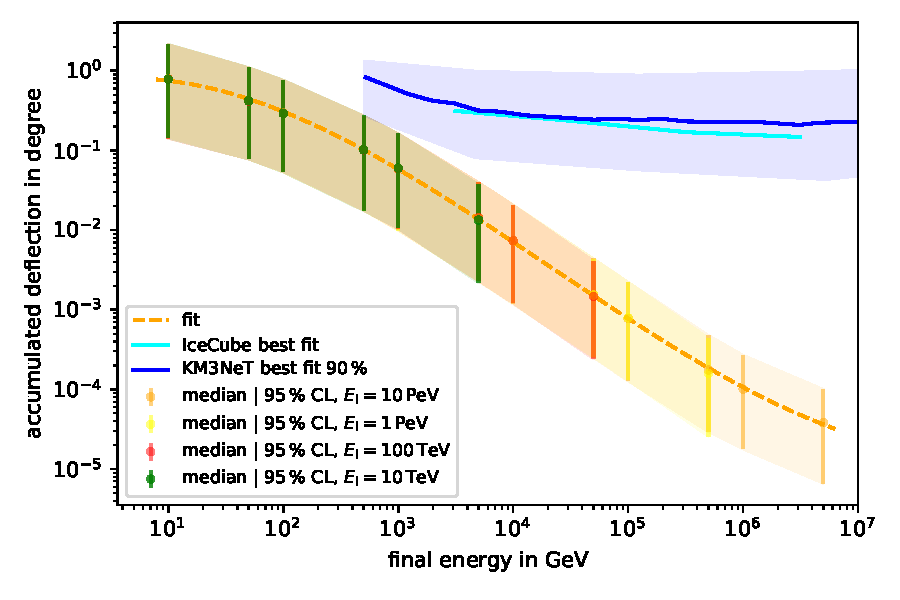
\includegraphics[width=\linewidth, height=.65\textheight, keepaspectratio]{plots/pascal.pdf}
    		  \captionsetup{justification=centering}
    		  \caption*{"NN-based parametrization of muon deflections simulated by PROPOSAL" \\ $\Rightarrow$ Talk \textbf{T46.6} by Pascal Gutjahr}
    		\end{figure}

        \end{column}
    \end{columns}
\end{frame}
